This chapter discusses tests the hypothesis stated in the Methodology chapter. To arrive at the hypothesis tests, this chapter will first discuss the descriptives of the dataset used for analysis (hereafter, the analysis dataset). Thereafter the research sub questions are investigated.
\section{Descriptive statistics}
Descriptive statistics are used to inform the reader about the general characteristics of the analysis dataset used to test the hypotheses. Preferably these characteristics resemble the characteristics of the wider population to allow for generalized statements. Therefore, the firms from analysis dataset were compared to the JSE All Share Index. The JSE All Share Index is the broad based Index of the Johannesburg Stock Exchange. The table below compares the sector weighting for the B-BBEE sample and the JSE All Share Index (equal weighted) as of latest date. The equal weight of latest date for the JSE All Share Index was retrieved from Thomson Reuters Datastream. This index comprised as of latest date because only the latest date (as of 30th April 2019) and names (no weight) were available for the constituents of the JSE All Share Index. The sector weighting for the B-BBEE sample was calculated by the following formula:
\begin{equation}
\begin{aligned}
W_{it} = \frac{N_{it}}{N_{t}}
\end{aligned}
\end{equation}
where, $W_{it}$ is the sector weight of sector $i$ at time $t$, $N_{it}$ is the number of firm in sector $i$ at time $t$ and $N_{t}$ is the total number of firms at time $t$. 

For the JSE All Share the time variable was fixed, as only the latest date was available. To check for bias in the B-BBEE sample, this study subtracted the weight per sector of  JSE All Share Index from the analysis dataset per sector per time. The result are displayed on the next.
\newpage
\begin{table}[H] %H forces the position of the table at the line where you place it (not on a separate page etc) -https://tex.stackexchange.com/questions/121155/how-to-adjust-a-table-to-fit-on-page https://tex.stackexchange.com/questions/332528/increasing-the-space-between-two-rows?rq=1
\centering
\caption{Relative bias sample versus JSE All Share Index 2019} 
\resizebox{\textwidth}{!}{\begin{tabular}{ccccccccc}

  \bottomrule
  \\
 Year & Basic Materials & Consumer Goods & Consumer Services & Financials   & Healthcare   & Industrials & Technology   & Telecommunications \\ \\
  \midrule
2004 & 6\%             & 0\%            & 5\%               & -18\%      & -3\%       & 4\%         & 4\%        & 1\%                \\
2005 & 2\%             & 2\%            & -2\%              & -14\%      & -1\%       & 4\%         & 8\%        & 1\%                \\
2006 & 2\%             & 4\%            & 1\%               & -18\%      & -1\%       & 1\%         & 9\%        & 1\%                \\
2007 & 4\%             & -3\%           & 1\%               & -9\%       & -1\%       & -2\%        & 9\%        & 1\%                \\
2008 & -3\%            & -5\%           & -5\%              & -11\%      & -1\%       & 9\%         & 13\%       & 3\%                \\
2009 & -8\%            & -1\%           & 1\%               & -11\%      & 1\%        & 11\%        & 9\%        & -2\%               \\
2010 & -8\%            & -3\%           & -2\%              & -14\%      & 1\%        & 14\%        & 9\%        & 3\%                \\
2011 & -6\%            & -3\%           & -5\%              & -13\%      & 1\%        & 16\%        & 8\%        & 3\%                \\
2012 & -4\%            & -5\%           & -4\%              & -13\%      & -1\%       & 16\%        & 9\%        & 1\%                \\
2013 & -6\%            & -3\%           & -4\%              & -11\%      & 1\%        & 11\%        & 8\%        & 4\%                \\
2014 & -8\%            & -1\%           & -5\%              & -13\%      & 1\%        & 14\%        & 8\%        & 4\%                \\
2015 & -9\%            & -3\%           & -4\%              & -8\%       & 1\%        & 16\%        & 8\%        & -1\%               \\
2016 & -3\%            & -5\%           & -10\%             & -9\%       & -4\%       & 23\%        & 8\%        & 1\%                \\
2017 & -3\%            & -6\%           & 13\%              & -31\%      & 2\%        & 26\%        & -1\%       & -1\%               \\
2018 & -3\%            & -5\%           & -4\%              & -14\%      & -1\%       & 19\%        & 8\%        & -1\%  \\ 
   \bottomrule
\end{tabular}}
\end{table} 
This table shows the percentage of observations in any of the respective sectors for the JSE All Share equal weight, and the firms for which B-BBEE rank was available. Recall that the JSE All Share equal weight was retrieved from one point in time, therefore the percentage of observations in any of the sectors of the JSE All Share equal weight was static through time. The constituents, and therefore the weight of each sector for analysis dataset used however did change annually.

Comparing the analysis dataset with the JSE All Share indicate bias towards Industrials. This might be due to the nature of this sector and relates to the cross sectional dynamics of the relationship between B-BBEE policy and firm performance as found in the theoretical framework. Most firms in the Industrial sector were active in the construction business. In the construction business, it is likely that a significant portion either directly or indirectly engages in business with government entities. Recall from the Theory chapter, that firms that reach B-BBEE targets receive B-BBEE aggregate score that places these firms eligible to obtain government business and/or business from firms that require suppliers to be B-BBEE compliant  (\citeauthor{N7}, \citeyear{N7}, p546; \citeauthor{N3}, \citeyear{N3}; \citeauthor{N5}, \citeyear{N5}, p9). The extraordinary benefit Industrials enjoy, especially compared to other sectors, could explain the bias of the Industrial sector in the analysis dataset. It is interesting to note the increase in bias toward the Industrial sector in this dataset compared to the JSE All Share equal weight adjustment of the B-BBEE policy. This relates to the time dynamics as found in the theoretical framework. Recall from the Contextualization chapter that amendments in B-BBEE policy occurred in 2007 and in 2013. Prior to 2007 the overrepresentation of Industrials was about 4\%, between 2007 and 2013 about 15\%, and after 2013 24\%.

Contrary, the analysis dataset underrepresented the Financials sector. This also could be explained from the cross-sectional dynamic standpoint. Financials, such as banks, could have a less obvious benefits of B-BBEE compliance as these firms are not directly tendering on government like Industrial firms. However, recall from the Theory that consumer behavior could reward firms that were exhibiting social responsible behaviour \cite[p378]{N34}. This is benefit is however not found significant enough in the case of the Financials sector in the analysis dataset. The underrepresentation is somewhat surprising as the Contextualization chapter revealed Sanlam, a Financials sector firm, was the first South African firm to implement a form of BEE by transferring 10\% of ownership to Black people. The underrepresentation leads speculation that firms operating in the Financial sector mostly engage in B-BBEE policy to minimize damage and therefore adopt a defensive and apprehensive strategy reflected in the underrepresentation of this sector in the analysis dataset.

Despite these difference, the top 3 dominant sectors of the JSE All Share equal weight; Basic Materials, Consumer Service and Financials are also dominant in the analysis dataset. The smaller sectors; Technology, Health Care and Telecommunication displayed at most overseeable deviations between the analysis dataset and JSE All Share Index. The JSE All Share Index consisted of 164 firms, of which 125 were included in the analysis dataset at some point in time. Therefore, the analysis dataset was found representative of Johannesburg Stock Exchange listed firms.

The maximum amount of observations, given 60 firms for 15 years equals 900. Below an overview of descriptive statistics for the variables for Model 1, the FF (Fama and French based) model using the analysis dataset.  
\begin{table}[H] %H forces the position of the table at the line where you place it (not on a separate page etc) -https://tex.stackexchange.com/questions/121155/how-to-adjust-a-table-to-fit-on-page https://tex.stackexchange.com/questions/332528/increasing-the-space-between-two-rows?rq=1
\centering
\caption{Descriptive statistics variables} 
\resizebox{\textwidth}{!}{\begin{tabular}{ccccccccc}

  \bottomrule
  \\
 & BMRatio    & SIZERatio  & EPRatio  & BPIndex\_YR1 & SIZEIndex\_YR1 & MarketPremium\_YR1 & RiskFreeReturn\_YR1 & SharePriceReturn\_YR1 \\ \\
  \midrule
count & 816   & 900     & 835      & 15           & 15             & 15                 & 15                  & 900                 \\
mean  & 0.90  & 36024   & -11.50   & 6\%          & 2\%            & 9\%                & 8\%                 & 14\%                \\
std   & 2.42  & 96943   & 221.03   & 6\%          & 7\%            & 23\%               & 1\%                 & 47\%                \\
min   & -0.47 & 3       & -4670.81 & 0\%          & -15\%          & -20\%              & 7\%                 & -95\%               \\
25\%  & 0.34  & 1522    & 5.10     & 3\%          & -1\%           & -5\%               & 8\%                 & -12\%               \\
50\%  & 0.55  & 7653    & 7.70     & 6\%          & 4\%            & 3\%                & 9\%                 & 10\%                \\
75\%  & 0.88  & 26091   & 10.30    & 8\%          & 8\%            & 18\%               & 9\%                 & 31\%                \\
max   & 55.66 & 1434027 & 65.39    & 23\%         & 12\%           & 67\%               & 10\%                & 756\%     \\ 
   \bottomrule
\end{tabular}}
\end{table} 
The one year forward share price return varied widely. The standard deviation was 47.6\%, and the difference between the minimum and maximum observation share price return for one year equaled more than 800\%. Similarly the BM ratio and SIZE ratio varied greatly. BM is the book to market ratio as defined by Merwe and Ferreira. The minimum BM ratio was negative, indicating a firm with negative book value. This indicates negative equity value, or a company in severe distress. The number of observations on the BM ratio equaled 816, indicating that of 900 observations there was no BM ratio available for 84 observations. SIZE ratio was the market capitalization as defined by Merwe and Ferreira. The SIZE ratio indicates that both very small firms and very large firms were available in the dataset used for analysis. The indices, BM, SIZE, MarketPremium, and RiskFreeReturn only showed 1 value for each year, hence 15 observations were yielded for these variables. The indices of BP, SIZE, MarketPremium and RiskFreeReturn are based upon the Fama and French methodology. Recall that the RiskFreeReturn equals 10 years South African government bond. The RiskFreeReturn remained, compared to the other variables,  relatively immune from variability. The bottom 25 percentile  observation equaled 8.1\% and the top 75 percentile observation equaled 8.7\%.

Given the large variability of some of the factors, this study adjusted analysis dataset for outliers (hereafter, outlier adjusted analysis dataset). The outlier adjusted analysis dataset constrained the minimum value for the BM ratio, SIZE ratio, EP ratio and share price return to -2 times standard deviation from the mean, and the maximum value to +2 times standard deviation from the mean. The descriptives for this outlier adjusted analysis dataset are presented below.
\begin{table}[H] 
\centering
\caption{Descriptive statistics variables outlier adjusted} 
\resizebox{\textwidth}{!}{\begin{tabular}{ccccccccc}
  \bottomrule
  \\
 & BMRatio    & SIZERatio   & EPRatio      & BPIndex\_YR1 & SIZEIndex\_YR1 & MarketPremium\_YR1 & RiskFreeReturn\_YR1 & SharePriceReturn\_YR1 \\ \\
  \midrule
count & 816   & 900    & 835      & 15           & 15             & 14                 & 14                  & 900                 \\
mean  & 0.77  & 29618  & -11.50   & 4\%          & 4\%            & 4\%                & 17\%                & 14\%                \\
std   & 0.79  & 52727  & 221.03   & 3\%          & 4\%            & 21\%               & 1\%                 & 40\%                \\
min   & -0.47 & 3      & -4670.81 & 0\%          & -3\%           & -27\%              & 15\%                & -95\%               \\
25\%  & 0.34  & 1522   & 5.10     & 2\%          & 1\%            & -7\%               & 17\%                & -12\%               \\
50\%  & 0.55  & 7653   & 7.70     & 4\%          & 3\%            & 1\%                & 18\%                & 10\%                \\
75\%  & 0.88  & 26091  & 10.30    & 6\%          & 6\%            & 7\%                & 18\%                & 31\%                \\
max   & 4.84  & 225857 & 65.39    & 11\%         & 12\%           & 50\%               & 19\%                & 189\%      \\
   \bottomrule
\end{tabular}}
\end{table} 
Recall that the indices of BM, SIZE and MarketPremium were based on the universe of share price returns available. Therefore, adjusting the share price return for outliers also impacted the indices of BM, SIZE and MarketPremium. The outlier adjusted analysis dataset still displayed variability, however at a much lower rate as can be viewed from the significantly lower maximum value for BMRatio, SIZERatio and share price return. It is interesting to note that the variability of the MarketPremium rose as result of the outlier adjustment for the share price return. This indicates that as outliers were excluded from share price return, correlations increased between firms share price return and therefore the variability of the MarketPremium increased.

The correlation matrix suggests that multicollinearity did not exist in the analysis dataset. Below the correlation matrix for the analysis dataset.
\begin{table}[H] 
\centering
\caption{Correlation matrix} 
\resizebox{\textwidth}{!}{\begin{tabular}{rrrrrrrrrr}
  \bottomrule
     & 1     & 2     & 3     & 4     & 5     & 6     & 7     & 8     & 9 \\
  \midrule
BMRatio (1)                  & 1.00  & -0.08 & -0.02 & 0.01  & -0.04 & -0.07 & 0.04  & 0.04  & -0.05 \\
SIZERatio (2)                & -0.08 & 1.00  & 0.03  & -0.03 & -0.05 & 0.06  & -0.04 & -0.06 & 0.04  \\
EPRatio (3)                 & -0.02 & 0.03  & 1.00  & 0.03  & -0.02 & 0.01  & 0.05  & 0.00  & 0.08  \\
BPIndex\_YR1 (4)        & 0.01  & -0.03 & 0.03  & 1.00  & 0.00  & -0.11 & -0.34 & 0.06  & -0.20 \\
BBBEE\_Rank (5)         & -0.04 & -0.05 & -0.02 & 0.00  & 1.00  & 0.00  & 0.00  & 0.00  & -0.03 \\
SIZEIndex\_YR1 (6)      & -0.07 & 0.06  & 0.01  & -0.11 & 0.00  & 1.00  & -0.60 & -0.28 & -0.15 \\
MarketPremium\_YR1 (7)  & 0.04  & -0.04 & 0.05  & -0.34 & 0.00  & -0.60 & 1.00  & -0.07 & 0.39  \\
RiskFreeReturn\_YR1 (8) & 0.04  & -0.06 & 0.00  & 0.06  & 0.00  & -0.28 & -0.07 & 1.00  & -0.05 \\
SharePriceReturn\_YR1 (9) & -0.05 & 0.04  & 0.08  & -0.20 & -0.03 & -0.15 & 0.39  & -0.05 & 1.00                 \\ 
   \bottomrule
\end{tabular}}
\end{table} 
An overview of the correlations on two, three, four and five years basis can be found in Appendix A. The correlation matrix for the outlier adjusted analysis dataset shows as similar picture, as can be viewed below.
\begin{table}[H] 
\centering
\caption{Correlation matrix} 
\resizebox{\textwidth}{!}{\begin{tabular}{rrrrrrrrrr}
  \bottomrule
     & 1     & 2     & 3     & 4     & 5     & 6     & 7     & 8     & 9 \\
  \midrule
BMRatio (1)                  & 1.00  & -0.23 & -0.08 & 0.02  & -0.02 & 0.03  & -0.10 & 0.06  & -0.17 \\
SIZERatio (2)                & -0.23 & 1.00  & 0.04  & 0.00  & -0.03 & 0.04  & -0.01 & -0.08 & 0.06  \\
EPRatio (3)                 & -0.08 & 0.04  & 1.00  & 0.05  & -0.02 & 0.04  & 0.05  & 0.00  & 0.09  \\
BPIndex\_YR1 (4)        & 0.02  & 0.00  & 0.05  & 1.00  & 0.00  & 0.53  & -0.34 & -0.12 & -0.16 \\
BBBEE\_Rank (5)         & -0.02 & -0.03 & -0.02 & 0.00  & 1.00  & 0.00  & 0.00  & 0.00  & -0.01 \\
SIZEIndex\_YR1 (6)      & 0.03  & 0.04  & 0.04  & 0.53  & 0.00  & 1.00  & -0.65 & -0.29 & -0.24 \\
MarketPremium\_YR1 (7)  & -0.10 & -0.01 & 0.05  & -0.34 & 0.00  & -0.65 & 1.00  & -0.27 & 0.46  \\
RiskFreeReturn\_YR1 (8) & 0.06  & -0.08 & 0.00  & -0.12 & 0.00  & -0.29 & -0.27 & 1.00  & -0.05 \\
SharePriceReturn\_YR1 (9) & -0.17 & 0.06  & 0.09  & -0.16 & -0.01 & -0.24 & 0.46  & -0.05 & 1.00                \\ 
   \bottomrule
\end{tabular}}
\end{table} 
Both correlation matrices indicate that there is no multicollinearity within the datasets. The observed correlations between the variables are low to negative. The correlation matrix for the outlier adjusted analysis dataset shows more pronounced correlations as expected. For example the correlation between BM ratio and SIZE ratio is -0.23 in the outlier adjusted analysis dataset versus -0.08 in the analysis dataset.

It can also be observed from the correlation matrix of the analysis dataset that the market, contrary intuition based on the Fama French theory, indicates a negative correlations between BM ratio and share price return and BM Index and share price return. Recall from the Theory chapter that Fama and French state that the market undervalues distressed, high book to market ratio firms, and therefore these firms tend to outperform low book to market ratio firms \cite[p1975]{N52}. This relationship is elusive in the analysis dataset. This indicates that this variable could be inappropriate to explain share price returns within the analysis dataset. On the other hand the correlation between MarketPremium and  share price return did display a higher correlation, 0.46. Therefore, the analysis dataset suggests that share price return for firms was mostly determined by movement of the general market. This, in the context of a developing/emerging market such as South Africa, seems perfectly logical as these markets are not as mature as the United States, Japanese or European markets upon which the Fama French study were based. Nonetheless the unexpected correlation between BM and share price return does raise concerns on the appropriateness of BM as a control variable in this study.
\section{Regression results}
Recall that the methodology indicated three aspects to the relationship between B-BBEE policy and firm performance, one calling for analysis the entire dataset, one calling for regression of specific time periods and one calling for regressions per sector. This section presents the empirical results of the regression analysis per sub research question by operationalizing B-BBEE policy through B-BBEE rank and firm performance with share price return, per specification in the Methodology chapter.
\subsection{Relationship between B-BBEE policy and firm performance 2004 -2018}
This section concerns the research sub question: “What was the long term relationship between  Broad-Based Black Economic Empowerment policy on firm performance of the Johannesburg Stock Exchange-listed companies over the period 2004 - 2018?”. The regression results of  analysis dataset for this sub research question for Model 1, the FF model (specified in the Methodology chapter) looks as follows:
\begin{table}[H] 
\tiny %https://tex.stackexchange.com/questions/27097/changing-the-font-size-in-a-table
\centering
\caption{Regression Model 1, 2004 - 2018} 
\resizebox{\textwidth}{!}{\begin{tabular}{lrrrrr}
  \bottomrule
     &     1     &     2     &     3      &     4     &     5      \\
  \midrule
BMIndex                 & -0.2480   & -0.4555   & -1.1840    & 0.3650    & 1.2904     \\
                   & (0.3197)  & (0.8511)  & (1.5824)   & (2.5089)  & (2.1644)   \\
BBBEE\_Rank         & -0.0006   & -0.0028*  & -0.0069*** & -0.0065*  & -0.0017    \\
                   & (0.0009)  & (0.0016)  & (0.0026)   & (0.0034)  & (0.0046)   \\
SIZEIndex               & 0.8076**  & 0.5197    & 0.6443     & 0.6603    & -0.1533    \\
                   & (0.3248)  & (0.5360)  & (0.7693)   & (1.1358)  & (1.1300)   \\
MarketPremium      & 0.9686*** & 1.0702*** & 1.1230***  & 1.4520*** & 1.6534***  \\
                   & (0.1079)  & (0.1748)  & (0.3680)   & (0.5178)  & (0.3945)   \\
RiskFreeReturn     & 0.6521    & -0.1951   & 0.8228     & -2.7341   & -4.1080    \\
                   & (2.2691)  & (2.9432)  & (3.6206)   & (7.5388)  & (7.9526)   \\
Consumer Goods     & 0.0369    & 0.2265    & 0.1400     & 1.7100    & 2.9063     \\
                   & (0.2143)  & (0.5548)  & (1.0675)   & (2.9893)  & (4.0711)   \\
Financials         & 0.0558    & 0.3282    & 0.3099     & 1.8070    & 2.9933     \\
                   & (0.2090)  & (0.5489)  & (1.0607)   & (2.9764)  & (4.0449)   \\
Technology         & -0.0488   & 0.2580    & 0.2805     & 1.8074    & 3.0038     \\
                   & (0.2127)  & (0.5551)  & (1.0666)   & (2.9762)  & (4.0513)   \\
Healthcare         & 0.0960    & 0.5821    & 0.5522     & 2.1466    & 3.4400     \\
                   & (0.2165)  & (0.5585)  & (1.0739)   & (2.9911)  & (4.0623)   \\
Industrials        & -0.0384   & 0.1635    & 0.0480     & 1.4233    & 2.2926     \\
                   & (0.2061)  & (0.5464)  & (1.0565)   & (2.9752)  & (4.0371)   \\
Consumer Services  & 0.0634    & 0.2392    & 0.1807     & 1.6321    & 2.7102     \\
                   & (0.2102)  & (0.5533)  & (1.0664)   & (2.9819)  & (4.0610)   \\
Basic Materials    & 0.0184    & 0.1657    & 0.0090     & 1.5287    & 2.4668     \\
                   & (0.2115)  & (0.5537)  & (1.0651)   & (2.9778)  & (4.0566)   \\
Telecommunications & 0.0742    & 0.2379    & 0.1742     & 1.5765    & 2.4642     \\
                   & (0.2201)  & (0.5583)  & (1.0682)   & (2.9831)  & (4.0483)   \\
N                  & 816       & 752       & 694        & 638       & 582        \\
R^2                 & 0.18      & 0.22      & 0.26       & 0.14      & 0.10       \\
   \bottomrule
Standard errors in parentheses.
* p<0.10, ** p<0.05, ***p0.01\
\end{tabular}}
\end{table} 
There are 5 columns visible in this table, these tables represent the share price returns time horizon. Therefore column 1 represent the 1 year share price return, column 2 represents the two year forward share price return, etc. From this model, under the specifications stated (no adjustment for outliers), r-squared for all time horizons exceed 0.10. Merwe and Ferreira (\citeyear{N7}, p551), in their study, note that a r-squared of 5.6\% is acceptable to investigate the relationship between B-BBEE score and share price return. Therefore, Model 1’s r-squared of equal to or exceeding 0.10, is interpreted as sufficient to capture the relationship between B-BBEE rank and share price return. 

Model 1 finds negative relationships between B-BBEE rank and share price return, significant on a two, three and four years time horizon. This means that for the specified time horizons, the better the B-BBEE rank, the worse the share price return. It has to be noted that the magnitude, especially compared to the coefficients of other independent variables is small. For example, the three year regression shows the most negative B-BBEE rank coefficient of -0.0069. This indicates that an 1 incremental improvement of B-BBEE rank results in a reduction on a two years share price return of merely 0.69\%. Recall from the descriptives section that the variability of share price return was quite high (non outlier adjusted standard deviation of 47\%), therefore the impact that a change in B-BBEE rank has on two years share price return is quite muted.  In comparison, the magnitude of the market premium is far larger, and significant over the five time horizons. This suggests that the impact of B-BBEE is relatively small, but negative. Merwe and Ferreira (\citeyear{N7}, p552) also observed a same small significant negative relationship between B-BBEE and share price return. Using the different time horizons, Model 1 adds to the finding of Merwe and Ferreira and shows that the negative coefficient of B-BBEE rank increases up until the 4 years time horizon, from -0.0006 to -0.065. The increase of magnitude follows suggestions by Mehta and Ward (\citeyear{N27}, p89) who indicated that the market has an initial response to a B-BBEE rank, which is more positive, and as the market processes information, the response to the B-BBEE rank becomes more pronounced. The negative increasing coefficient and significance of the relationship between B-BBEE rank and share price performance over various share price return time horizons indicate that the costs of B-BBEE policy compliance for firm outweigh the benefits, causing a negative long term relationship between B-BBEE policy and firm performance.

To check for robustness, the same model was tested on the outlier adjusted analysis dataset. Below the results.
\newpage
\begin{table}[t] 
\tiny %https://tex.stackexchange.com/questions/27097/changing-the-font-size-in-a-table
\centering
\caption{Regression Model 1 - outlier adjusted, 2004 - 2018} 
\resizebox{\textwidth}{!}{\begin{tabular}{lrrrrr}
  \bottomrule
     &     1     &     2     &     3      &     4     &     5      \\
  \midrule
BMIndex                 & -0.4858   & -1.8037   & -2.0434   & -2.5375*  & -1.0682   \\
                   & (0.4961)  & (1.2019)  & (1.5805)  & (1.4165)  & (1.7208)  \\
BBBEE\_Rank         & 0.0002    & -0.0023*  & -0.0040** & -0.0046** & -0.0031   \\
                   & (0.0008)  & (0.0012)  & (0.0018)  & (0.0023)  & (0.0031)  \\
SIZEIndex               & 1.4892*** & 1.4440*** & 1.9992*** & 1.5684*   & 0.7834    \\
                   & (0.5035)  & (0.4597)  & (0.5777)  & (0.8307)  & (1.2044)  \\
MarketPremium      & 0.9909*** & 0.7264*** & 0.5739    & 0.6428    & 0.9448**  \\
                   & (0.0889)  & (0.2324)  & (0.4437)  & (0.3912)  & (0.3946)  \\
RiskFreeReturn     & -0.9639   & -5.2936** & -6.9621** & -3.7378   & -4.6235   \\
                   & (2.3277)  & (2.4482)  & (3.0451)  & (2.5987)  & (3.0165)  \\
Consumer Goods     & 0.1620    & 1.1208*** & 2.2522*** & 2.0092**  & 3.1361**  \\
                   & (0.2098)  & (0.4083)  & (0.7774)  & (0.9581)  & (1.4945)  \\
Financials         & 0.1339    & 1.1070*** & 2.1980*** & 1.9381**  & 3.0821**  \\
                   & (0.2058)  & (0.4012)  & (0.7659)  & (0.9435)  & (1.4760)  \\
Technology         & 0.0557    & 1.0409**  & 2.0749*** & 1.5954*   & 2.5532*   \\
                   & (0.2091)  & (0.4069)  & (0.7730)  & (0.9501)  & (1.4821)  \\
Healthcare         & 0.2218    & 1.3349*** & 2.5125*** & 2.3881**  & 3.7449**  \\
                   & (0.2115)  & (0.4115)  & (0.7734)  & (0.9552)  & (1.4895)  \\
Industrials        & 0.0540    & 0.9886**  & 1.9611**  & 1.5478*   & 2.4982*   \\
                   & (0.2035)  & (0.3977)  & (0.7609)  & (0.9391)  & (1.4675)  \\
Consumer Services  & 0.1520    & 1.1381*** & 2.2232*** & 1.8841**  & 2.9608**  \\
                   & (0.2070)  & (0.4056)  & (0.7723)  & (0.9489)  & (1.4848)  \\
Basic Materials    & 0.1664    & 1.0613*** & 2.1641*** & 1.7577*   & 2.7730*   \\
                   & (0.2072)  & (0.4061)  & (0.7780)  & (0.9528)  & (1.4871)  \\
Telecommunications & 0.1557    & 1.1154*** & 2.2015*** & 1.7467*   & 2.6537*   \\
                   & (0.2129)  & (0.4132)  & (0.7783)  & (0.9564)  & (1.4832)  \\
N                  & 757       & 693       & 635       & 579       & 523       \\
R^2                 & 0.24      & 0.20      & 0.14      & 0.15      & 0.14      \\
   \bottomrule
Standard errors in parentheses.
* p<0.10, ** p<0.05, ***p<0.01
\end{tabular}}
\end{table} 
Here the relationship between B-BBEE rank and share price return on a one-year time horizon is slightly positive albeit not significant. On the two, three and four years time horizon, the relationship between B-BBEE rank and share price returns remains, just as in the analysis dataset,  negative and significant, but at slightly less negative coefficient compared to the analysis dataset. In contrast the 5 years time horizon displays a more pronounced negative coefficient, compared to the non outlier adjusted model. Therefore, the outlier adjusted Model 1 suggest that outliers did indeed impact the analysis dataset. However, the finding from Model 1 for the analysis dataset, displaying significant negative relationships between B-BBEE rank and share price return on various time horizons remained intact.
\newpage
Using the Model 2, based on the Merwe and Ferreira model the analysis dataset yields the following results:
\begin{table}[H] 
\tiny %https://tex.stackexchange.com/questions/27097/changing-the-font-size-in-a-table
\centering
\caption{Regression Model 2, 2004 - 2018} 
\resizebox{\textwidth}{!}{\begin{tabular}{lrrrrr}
  \bottomrule
     &     1     &     2     &     3      &     4     &     5      \\
  \midrule
const              & 0.1734*** & 0.3719*** & 0.6843*** & 0.8264*** & 0.8976***  \\
                   & (0.0343)  & (0.0633)  & (0.1052)  & (0.1258)  & (0.1680)   \\
BMRatio                 & -0.0078   & 0.0452*** & 0.0617*** & 0.0560**  & 0.0518*    \\
                   & (0.0071)  & (0.0125)  & (0.0201)  & (0.0232)  & (0.0296)   \\
SIZERatio               & 0.0000    & -0.0000   & -0.0000*  & -0.0000   & -0.0000    \\
                   & (0.0000)  & (0.0000)  & (0.0000)  & (0.0000)  & (0.0000)   \\
EPRatio                & 0.0001*   & 0.0006*** & 0.0006*   & 0.0007*   & 0.0027*    \\
                   & (0.0001)  & (0.0002)  & (0.0003)  & (0.0004)  & (0.0014)   \\
BBBEE\_Rank         & -0.0004   & -0.0024   & -0.0065** & -0.0068*  & -0.0016    \\
                   & (0.0010)  & (0.0018)  & (0.0030)  & (0.0036)  & (0.0048)   \\
Consumer Goods     & 0.0562    & 0.1012    & 0.1306    & 0.1914    & 0.2939     \\
                   & (0.0573)  & (0.1038)  & (0.1694)  & (0.2020)  & (0.2689)   \\
Financials         & 0.0388    & 0.0791    & 0.1678    & 0.2121    & 0.2970*    \\
                   & (0.0363)  & (0.0653)  & (0.1084)  & (0.1305)  & (0.1744)   \\
Technology         & -0.0606   & -0.0277   & 0.0457    & 0.1290    & 0.3067     \\
                   & (0.0525)  & (0.0934)  & (0.1542)  & (0.1832)  & (0.2435)   \\
Healthcare         & 0.0550    & 0.3260**  & 0.3339    & 0.4978*   & 0.7604**   \\
                   & (0.0761)  & (0.1421)  & (0.2277)  & (0.2754)  & (0.3714)   \\
Industrials        & -0.0838** & -0.1404** & -0.1430   & -0.1942   & -0.3659**  \\
                   & (0.0363)  & (0.0674)  & (0.1136)  & (0.1371)  & (0.1833)   \\
Consumer Services  & 0.0507    & 0.0393    & 0.0932    & 0.0534    & 0.0341     \\
                   & (0.0441)  & (0.0839)  & (0.1367)  & (0.1621)  & (0.2140)   \\
Basic Materials    & 0.0523    & -0.0467   & -0.0752   & -0.1002   & -0.2772    \\
                   & (0.0456)  & (0.0834)  & (0.1389)  & (0.1633)  & (0.2147)   \\
Telecommunications & 0.0647    & 0.0411    & 0.1312    & 0.0371    & -0.1515    \\
                   & (0.0828)  & (0.1491)  & (0.2471)  & (0.2904)  & (0.3949)   \\
N                  & 816       & 752       & 694       & 638       & 582        \\
R^2                 & 0.02      & 0.04      & 0.04      & 0.03      & 0.04       \\
   \bottomrule
Standard errors in parentheses.
* p<0.10, ** p<0.05, ***p<0.01
\end{tabular}}
\end{table} 
It is immediately visible that the r-squared of Model 2 which follows the Merwe and Ferreira model lags the Model 1 which followed the Fama French model more closely. This strengthens the belief that the control variables as used in the Fama French model are more appropriate to explain share price return. Model 1 is significant on two, three and four years returns and Model 2  is significant on three and four years. Merwe and Ferreira (\citeyear{N7}, p552) use B-BBEE score rather than B-BBEE rank and found a coefficient of -0.003 at 1\% significant between B-BBEE score and share price return. The Merwe and Ferreira finding means that an one increment increase of B-BBEE score detracts 0.30\% of one year share price return. This coefficient differs from the finding presented in this study, when comparing this finding with the 1 year time horizon model as this study finds a (insignificant) coefficient nearly close to zero, -0.0004. This difference could arise from time period bias in the Merwe and Ferreira research as Merwe and Ferreira use the time period of 2005 - 2011, whereas this study analyzes the time period 2004 - 2018.

Nonetheless, the findings of Model 2 on the relationship between B-BBEE rank and share price return are largely unchanged. The coefficients for the relationship between B-BBEE rank and share price return at most differ -0.0004. This means that for the entire time period of 2004 to 2018 a higher B-BBEE rank did not add to share price returns.
\subsection{Relationship between B-BBEE policy on firm performance in three B-BBEE policy periods}
This section deals with the research sub question: “What was the relationship between B-BBEE policy and firm performance among the three B-BBEE policy periods?”. Previous research on the relationship between B-BBEE and firm performance did not show consensus on the nature of the relationship. This could be due to the different time periods the studies used. It could be that the overall nature between B-BBEE and firm performance was negative, but that a particular time periods the relationship was positive. It could also be that the negative relationship over the entire dataset found in the previous section is driven by a particular time period. This study examined the relationship over the three periods of B-BBEE, as explained in the Methodology. The three sections this study identified where from 2004 until 2007, from 2007 until 2013 and from 2013 until 2018. These sections were selected based on B-BBEE policy initiation in 2004 and B-BBEE policy amendments in 2007 and 2013. Below the relationships between B-BBEE rank and share price returns over the three periods.

The period 2004 to 2007 shows the following regression results for the analysis dataset using Model 1:
\begin{table}[H] 
\tiny %https://tex.stackexchange.com/questions/27097/changing-the-font-size-in-a-table
\centering
\caption{Regression Model 1, sub sections} 
\resizebox{\textwidth}{!}{\begin{tabular}{lrrrrr}
  \bottomrule
     &     1     &     2     &     3      &     4     &     5      \\
  \midrule
BBBEE\_Rank 2004 - 2007        & -0.0036  & 0.0032   & -0.0066  & -0.0084  & -0.0028    \\
                   & (0.0032) & (0.0055) & (0.0081) & (0.0073) & (0.0067)   \\
BBBEE\_Rank 2007 - 2013        & 0.0009    & -0.0030  & -0.0054*  & -0.0033   & 0.0008     \\
                   & (0.0009)  & (0.0019) & (0.0032)  & (0.0050)  & (0.0070)   \\
BBBEE\_Rank 2013 - 2018       & -0.0002   & -0.0060*** & -0.0083*** & -0.0123*** & -0.0088    \\
                   & (0.0013)  & (0.0020)   & (0.0030)   & (0.0040)   & (0.0061)   \\                   
   \bottomrule
Standard errors in parentheses.
* p<0.10, ** p<0.05, ***p<0.01
\end{tabular}}
\end{table} 
The period 2004 - 2007 shows no significant relationship between between B-BBEE rank and share price return. Recall from the chronology discussed in earlier section that this was a period in which B-BBEE policy was not enforced tightly. The results over time do display that increasing interventionist stance of the B-BBEE became more pronounced in share price return. the relationship between B-BBEE rank and one and five year share price return were marginally positive. With regards to the 2007 to 2013 period, the relationship between B-BBEE and share price returns on two, three and four years basis were less negative compared to the entire dataset results. It has to be noted that these findings, with the exception of the three years regression, were not significant. These findings resemble the findings of Mokgobinyane who found a disperse relationship between the B-BBEE score coefficients on different measurements of firm performance using observations from this time period. Finally, with regards to the 2013 to 2018 period, it is found that this time period produces the most pronounced negative relationships between B-BBEE rank and share price return. The negative coefficients of B-BBEE rank on the two, three and four years share price return were found significant on 1\%. The descriptive statistics section of this chapter, this study observed that the bias toward Industrials, a sector more dependent on B-BBEE compliance, increased as the Codes of Practise became more stringent over time. However, this study finds that the benefits of B-BBEE compliance over the 2013 to 2018 did not outweigh the costs. This finding contrasts Acemoglu et al. (\citeyear{N23}, p32), who finds positive, but not significant, relationship between B-BBEE aggregate score and net profit margin. It could be however, especially consider the short time span, that a disconnect existed between net profit margins and share price returns. For example, Merwe and Ferreira (\citeyear{N7}, p552)  examined the period 2005 to 2011, which therefore overlaps the period 2004 to 2007 and found a small significant negative relationship between B-BBEE and share price return. The analysis of the different sub-sections of time indicate that increasing intervention of B-BBEE policy caused a more pronounced negative relationship between B-BBEE policy and share price return.
\subsection{Relationship between B-BBEE policy on firm performance on sector basis}
The theoretical framework also identified cross-sectional dynamics to hypothetically affect the relationship between B-BBEE policy. The theory notes that the aggregate cost and benefit for firms to comply to the B-BBEE policy might differ across sectors. This relates to the sub research question: “Did the relationship between B-BBEE policy and firm performance differ across sectors?”. Therefore the analysis dataset was subdivided per sector. The next table displays result of the sector linear regressions using Model 1 per sector.
\begin{table}[H] 
\tiny %https://tex.stackexchange.com/questions/27097/changing-the-font-size-in-a-table
\centering
\caption{Regression Model 1, sub sections} 
\resizebox{\textwidth}{!}{\begin{tabular}{lrrrrr}
  \bottomrule
     &     1     &     2     &     3      &     4     &     5      \\
  \midrule
BBBEE\_Rank\_Telecom      & -0.0012  & 0.0006     & -0.0005    & -0.0082    & -0.0221   \\
                          & -0.0041  & -0.0075    & -0.0107    & -0.0132    & -0.0191   \\
BBBEE\_Rank\_BasicMat     & 0.0007   & -0.0008    & -0.0045    & -0.011     & -0.009    \\
                          & -0.0031  & -0.0049    & -0.0067    & -0.0078    & -0.0083   \\
BBBEE\_Rank\_ConsumerServices & 0.0019   & -0.001     & -0.0042    & -0.0069    & -0.0094   \\
                          & -0.0014  & -0.0025    & -0.0036    & -0.0056    & -0.0067   \\
BBBEE\_Rank\_Industrials  & -0.0027* & -0.0125*** & -0.0182*** & -0.0201*** & -0.0132*  \\
                          & -0.0016  & -0.0027    & -0.0047    & -0.006     & -0.007    \\
BBBEE\_Rank\_HealthCare   & -0.0005  & 0.0069     & -0.0016    & 0.0052     & 0.0084    \\
                          & -0.0039  & -0.0095    & -0.0087    & -0.0098    & -0.0214   \\
BBBEE\_Rank\_Technology   & 0.0012   & -0.0042    & -0.0009    & 0.014      & 0.0365    \\
                          & -0.0033  & -0.0076    & -0.0141    & -0.0237    & -0.0363   \\
BBBEE\_Rank\_Financials   & -0.0019  & 0.0024     & 0.0012     & 0.0041     & 0.0071    \\
                          & -0.0022  & -0.0039    & -0.0064    & -0.0068    & -0.0091   \\
BBBEE\_Rank\_ConsumerGoods & 0.0011   & 0.0053**   & 0.0024     & 0.0032     & 0         \\
                          & -0.0019  & -0.0026    & -0.0038    & -0.0047    & -0.0068   \\
                          &          &            &            &            &           \\
N\_Telecom                & 32       & 30         & 28         & 27         & 23        \\
N\_BasicMat               & 117      & 101        & 93         & 89         & 84        \\
N\_ConsumerServices           & 124      & 100        & 97         & 90         & 84        \\
N\_Industrials            & 221      & 179        & 158        & 141        & 125       \\
N\_HealthCare             & 35       & 29         & 29         & 26         & 23        \\
N\_Technology             & 91       & 84         & 78         & 72         & 66        \\
N\_Financials             & 215      & 197        & 180        & 162        & 147       \\
N\_ConsumerGoods           & 215      & 197        & 180        & 162        & 147         \\                   
   \bottomrule
Standard errors in parentheses.
* p<0.10, ** p<0.05, ***p<0.01
\end{tabular}}
\end{table} 
The sectors Consumer Goods, Technology, Health Care and Telecom have less than 100 observations on one year time horizon. Considering 15 years, that means that these sector could exhibit time period bias. The Model 1 for these sectors are mostly insignificant with varying coefficients. Only the Consumer Goods sector on a two years horizon shows significant negative relationship between B-BBEE policy and firm performance. However, due to the insignificance of most relationships and the low observation count, it is difficult to state substantial claims based on these sectors.

The relationship between B-BBEE policy and firm performance for Financials is found insignificant but positive. This contradicts suspicions raised in the descriptive statistics section, where underrepresentation towards Financials hinted towards possible low benefits of B-BBEE compliance to Financials. This finding of insignificant but positive relationship between B-BBEE policy and firm performance for this sector could hint that firms that do decide to comply to B-BBEE policy find that benefits are greater than costs. This insignificant positive relationship demands further investigation.

Most interestingly, the sectors in which the incentives to comply, access to government contracts, was expected larger, display negative relationship between B-BBEE policy and firm performance. Most notable, the Industrial sector shows highly significant and most pronounced negative coefficients. This indicates that the benefits presented for these firm to comply to B-BBEE policy are underwhelming compared to the costs. It is further interesting to note that for Industrial to coefficient becomes more pronounced negative as time horizon increases, until the four year time horizon. This indicates that especially on the longer term the relationship between B-BBEE policy and firm performance is negative and favors the notion from the Theory that the incentive to comply to B-BBEE by providing access is, acts more as a cost to continue to do business. 
\section{Bootstrap method}
To add robustness to the findings from the regression analysis, this study investigated whether the relationship between B-BBEE rank and share price return displayed a deviating result using the Bootstrap method as stated by Mehta and Ward. This adds robustness to answer the research sub questions “What was the long term relationship between Broad-Based Black Economic Empowerment policy on firm performance of the Johannesburg Stock Exchange-listed companies over the period 2004 - 2018?” and  “Did the relationship between B-BBEE policy and firm performance differ across sectors?”. Next, a visualization of the bootstrap method results.
\newpage
\begin{figure}[H]
  \centering
  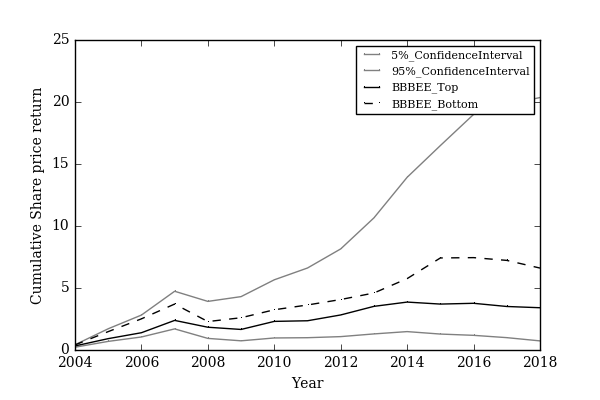
\includegraphics [scale=0.75]{Images/Bootstrap_All.png} \\
  {\small {\it \caption{Bootstrap entire dataset \label{fig:moun} }}}
\end{figure}
This chart displays four variables the 5\% and 95\% confidence intervals and the share price return of the top and bottom B-BBEE ranking firms. The confidence intervals were generated by bootstrapping the average returns of the entire dataset for each year, and retrieving the 5\% lowest and 5\% highest average returns for this year. These returns, as well as the returns for the top and bottom B-BBEE ranking firms were compounded over time. The top and bottom B-BBEE ranking firms were the average return of top and bottom 30\% ranking firms for each years. This chart shows that the 5\% highest average returns, the 95\% confidence interval rose significantly post 2008, outperforming all other variables handsomely as the average returns compounded aggressively. Similarly, although at a significant smaller compounding rate, the bottom B-BBEE ranking firms rose after 2008. It is particularly striking that from this analysis the bottom ranking B-BBEE firms outperform the top ranking B-BBEE firms. This analysis further shows the the bottom ranking B-BBEE firms do outperform the 5\% low confidence interval. This indicates the relationship between B-BBEE and share price return is insignificant, but most likely negative. Therefore this analysis provides (weak) support to the finding of the regression analyses on the entire period 2004 to 2018.

Returning towards a possible bias in the Industrial sector, this study performed the same bootstrap analysis for firms in this sector to answer the sub question: “Did firms operating in a sector with a higher incentive to comply to the B-BBEE policy have higher firm performance?” Next a visualization of the results. 
\newpage
\begin{figure}[H]
  \centering
  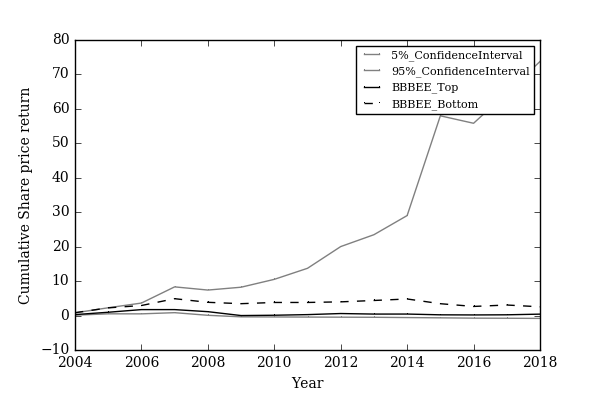
\includegraphics [scale=0.75]{Images/Bootstrap_Industrials.png} \\
  {\small {\it \caption{Bootstrap Industrials \label{fig:moun} }}}
\end{figure}
The above bootstrap analysis on the Industrial sector did entail a smaller sample size, which might explain that the findings of this chart are an exaggeration of the findings in the bootstrap analysis on the entire dataset. This chart, contrary to the idea in the Descriptives section, it appears that the negative relationship between B-BBEE and share price return is close to significant, as the top B-BBEE ranking firms in the Industrial sector remain close to the bottom 5\% confidence interval. This confirms earlier findings from the regression analysis on a sector by sector basis. 

The simulation for Consumer Services also shows a non significant performance of the top ranking B-BBEE firms. This can be seen below.
\begin{figure}[H]
  \centering
  \includegraphics [scale=0.75]{"Images/Bootstrap_Consumer Services_Cumulative"} \\
  {\small {\it \caption{Bootstrap Consumer Services \label{fig:moun} }}}
\end{figure}
This sector, however, does display that the top ranking B-BBEE firms outperformed the bottom ranking B-BBEE firms. Recall, from the Theory states that  consumer behavior could express their values regarding empowerment in their consumption pattern \cite[p378]{N34}. This chart shows weak evidence of this statement. This effect supports the Financial sector regression finding that firms with no direct or indirect government access could benefit from B-BBEE policy compliance.

The other sector bootstrap simulation can be found in Appendix C. Note however, that the sectors Telecommunications, Technology, Health Care and Consumer Goods had only a limited number of observations in each year. This could affect the robustness of the findings per sector. 
\section{Summary and conclusion}
Descriptive statistics were used to inform the reader about the general characteristics of the dataset used to test the hypothesis. These displayed a sizeable sample size, with at most 816 observations. Furthermore, the sample size did display a positive bias towards the Industrial sector and a negative bias towards the Financial sector, which, this study speculates, could be attributed to the sector’s incentive to comply to B-BBEE relating to market access.

Although the dataset did present outliers, the outliers did not meaningfully alter the conclusions on the regression analyses used to answer the research sub question: “What was the long term relationship between Broad-Based Black Economic Empowerment policy on firm performance of the Johannesburg Stock Exchange-listed companies over the period 2004 - 2018?”. Both outlier and non outlier adjusted regressions of Model 1, the FF model, indicate that the relationship between B-BBEE rank and two, three and four years share price return  was significantly negative. Model 2, the MF model, confirmed the finding on three and four years share price return. The significance levels did differ. For example, the non-outlier adjusted model 1 was significant at 1\% on 3 years share price return, whereas model 2 for this time horizon was significant at 5\%. Further, Model 2, the  MF model, held quite low explanatory value, with r squared below 5\%, whereas Model 1, the FF model generated acceptable r-squared equal to or larger than 14\%. This means that the better a firm complies to B-BBEE policy in the long term, the worse it share price return will be. This notion was supported, albeit not significantly, as the bootstrap method confirmed outperformance of firms that whose compliance to B-BBEE policy was weak, over firms whose compliance to B-BBEE policy was good. Therefore the hypothesis The relationship between B-BBEE policy and firm performance between 2004 and 2018 was positive was rejected.

Regressions were tested on sub sections of the dataset to answer the research sub question: “What was the long term relationship between B-BBEE policy and firm performance among the three B-BBEE policy periods?”. The results over time do display that increasing interventionist stance of the B-BBEE became more pronounced in share price return. The period 2013-2018 displayed more pronounced significant negative relationship between B-BBEE and two, three and four years share price return compared to the entire dataset. Further the strength of the 2013-2018 subset, measured in the coefficient of the B-BBEE rank on share price return, was more pronounced than period 2007-2013 and the 2004 to 2007 period on a two, three and four years time horizon. Therefore, this study speculates, that the increased targets aggravated costs and therefore the aggregate effect of B-BBEE policy on firm performance became more pronounced negative. In either case, the hypothesis The intensity of the relationship between B-BBEE policy and firm performance is uniform through time is rejected.

Finally, empirical analysis was done to explore the cross-sectional dimension of the relationship between B-BBEE policy and firm performance in the long term. This related to the research sub question “Did the relationship between B-BBEE policy and firm performance differ across sectors?”. The descriptives, as mentioned, already hinted towards cross sectional effects. The regression analysis per sector proved that the long term relationship for Industrials was most pronounced, with coefficients of B-BBEE rank significantly negative. The bootstrap provided weak support to this finding. This study speculates that these findings support the notion coined in the Theory chapter that the benefit of market access through B-BBEE policy compliance, actually acts more as a tax to continue business with government entities. The hypothesis The relationship between B-BBEE policy and firm performance is uniform across sectors is rejected.
